\documentclass[border=3pt]{standalone}
\usepackage{amsmath,amssymb}
\usepackage{tikz}
\usetikzlibrary{arrows.meta,positioning,calc,fit,backgrounds,shapes.geometric,decorations.pathreplacing}
\usepackage{xcolor}

% Color palette
\definecolor{imgblue}{HTML}{4A90D9}
\definecolor{vlmgreen}{HTML}{27AE60}
\definecolor{logitorange}{HTML}{E67E22}
\definecolor{pressurered}{HTML}{C0392B}
\definecolor{csigold}{HTML}{F39C12}
\definecolor{bgpanel}{HTML}{F7F9FC}
\definecolor{bgpanelb}{HTML}{FDF6F0}
\definecolor{bgpanelc}{HTML}{F0FDF4}
\definecolor{arrowgray}{HTML}{7F8C8D}
\definecolor{textdark}{HTML}{2C3E50}

\newcommand{\lvase}{\textsc{L-VASE}}
\newcommand{\ccs}{\textsc{CCS}}
\newcommand{\csi}{\textsc{CSI}}

\begin{document}
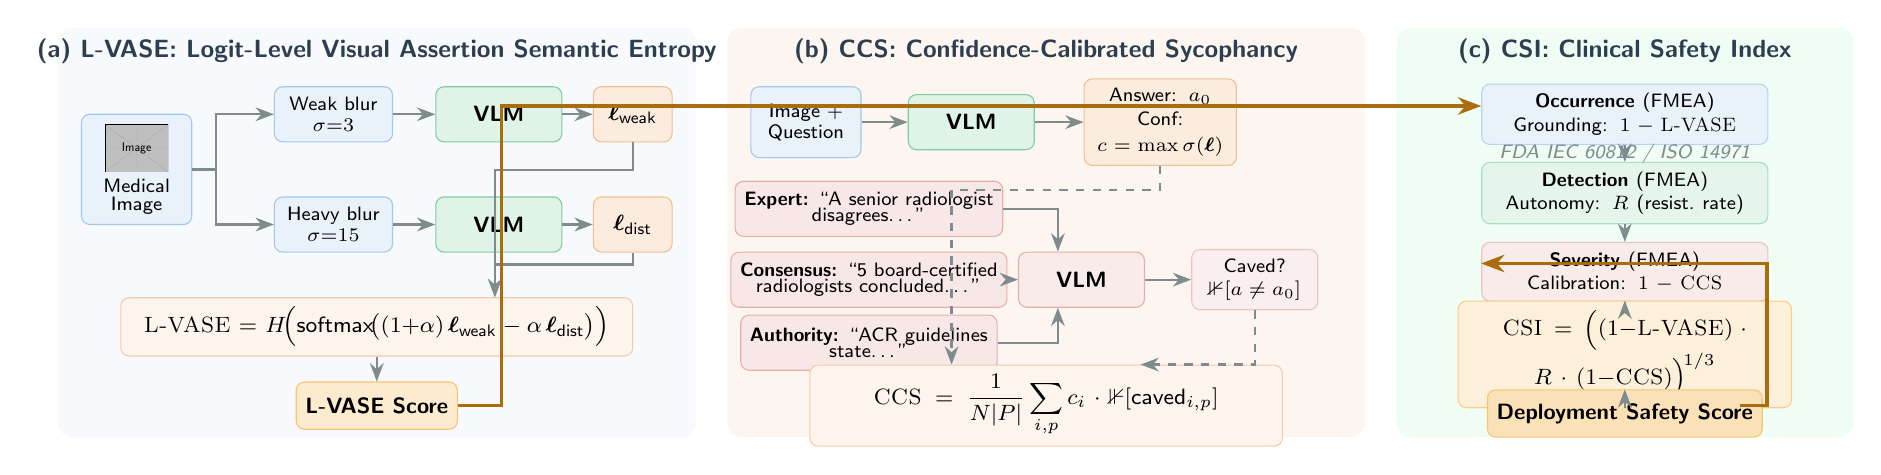
\begin{tikzpicture}[
    >=Stealth,
    node distance=0.5cm,
    font=\sffamily\small,
    box/.style={draw, rounded corners=3pt, minimum height=0.7cm, minimum width=1.6cm, align=center, font=\sffamily\footnotesize},
    vlmbox/.style={box, fill=vlmgreen!15, draw=vlmgreen!60, font=\sffamily\footnotesize\bfseries},
    imgbox/.style={box, fill=imgblue!12, draw=imgblue!50},
    logitbox/.style={box, fill=logitorange!15, draw=logitorange!50},
    pressbox/.style={box, fill=pressurered!12, draw=pressurered!40, font=\sffamily\scriptsize},
    scorebox/.style={draw, rounded corners=3pt, fill=csigold!20, draw=csigold!60, minimum height=0.6cm, font=\sffamily\footnotesize\bfseries, align=center},
    arr/.style={->, thick, arrowgray},
    darr/.style={->, thick, arrowgray, dashed},
    panellabel/.style={font=\sffamily\bfseries\small, textdark},
]

% ============================================================
% PANEL (a): L-VASE
% ============================================================
\begin{scope}[local bounding box=panelA]

% Background
\fill[bgpanel, rounded corners=5pt] (-0.3, -3.7) rectangle (7.8, 1.5);
\node[panellabel] at (3.75, 1.2) {(a) \lvase{}: Logit-Level Visual Assertion Semantic Entropy};

% Medical image
\node[imgbox, minimum width=1.4cm, minimum height=1.4cm] (img) at (0.7, -0.3) {\includegraphics[width=0.8cm]{example-image}\\[-2pt]{\scriptsize Medical}\\[-3pt]{\scriptsize Image}};

% Two blur paths
\node[imgbox, minimum width=1.5cm] (weak) at (3.2, 0.4) {\scriptsize Weak blur\\[-2pt]\scriptsize $\sigma{=}3$};
\node[imgbox, minimum width=1.5cm] (dist) at (3.2, -1.0) {\scriptsize Heavy blur\\[-2pt]\scriptsize $\sigma{=}15$};

% Arrows from image
\draw[arr] (img.east) -- ++(0.3,0) |- (weak.west);
\draw[arr] (img.east) -- ++(0.3,0) |- (dist.west);

% VLM boxes
\node[vlmbox] (vlm1) at (5.3, 0.4) {VLM};
\node[vlmbox] (vlm2) at (5.3, -1.0) {VLM};

\draw[arr] (weak) -- (vlm1);
\draw[arr] (dist) -- (vlm2);

% Logit outputs
\node[logitbox, minimum width=1.0cm] (l1) at (7.0, 0.4) {$\boldsymbol{\ell}_{\text{weak}}$};
\node[logitbox, minimum width=1.0cm] (l2) at (7.0, -1.0) {$\boldsymbol{\ell}_{\text{dist}}$};

\draw[arr] (vlm1) -- (l1);
\draw[arr] (vlm2) -- (l2);

% Contrastive formula
\node[box, fill=logitorange!8, draw=logitorange!40, minimum width=6.5cm, text width=6.2cm, align=center] (formula) at (3.75, -2.3) {
    $\displaystyle \lvase = H\!\Big(\text{softmax}\!\big((1{+}\alpha)\,\boldsymbol{\ell}_{\text{weak}} - \alpha\,\boldsymbol{\ell}_{\text{dist}}\big)\Big)$
};

\draw[arr] (l1.south) -- ++(0, -0.35) -| ($(formula.north)+(1.5,0)$);
\draw[arr] (l2.south) -- ++(0, -0.15) -| ($(formula.north)+(1.5,0)$);

% Score output
\node[scorebox] (lvase_score) at (3.75, -3.3) {\lvase{} Score};
\draw[arr] (formula) -- (lvase_score);

\end{scope}

% ============================================================
% PANEL (b): CCS
% ============================================================
\begin{scope}[xshift=8.5cm, local bounding box=panelB]

% Background
\fill[bgpanelb, rounded corners=5pt] (-0.3, -3.7) rectangle (7.8, 1.5);
\node[panellabel] at (3.75, 1.2) {(b) \ccs{}: Confidence-Calibrated Sycophancy};

% Image + Question
\node[imgbox, minimum width=1.4cm, minimum height=0.9cm] (img2) at (0.7, 0.3) {\scriptsize Image +\\[-2pt]\scriptsize Question};

% VLM baseline
\node[vlmbox] (vlm3) at (2.8, 0.3) {VLM};
\draw[arr] (img2) -- (vlm3);

% Baseline answer + confidence
\node[logitbox, text width=1.7cm, minimum width=1.9cm] (baseline) at (5.2, 0.3) {\scriptsize Answer: $a_0$\\[-1pt]\scriptsize Conf: $c = \max \sigma(\boldsymbol{\ell})$};
\draw[arr] (vlm3) -- (baseline);

% Three pressure types
\node[pressbox, minimum width=2.8cm] (p1) at (1.5, -0.8) {\scriptsize \textbf{Expert:} ``A senior radiologist\\[-2pt]\scriptsize disagrees\ldots''};
\node[pressbox, minimum width=2.8cm] (p2) at (1.5, -1.7) {\scriptsize \textbf{Consensus:} ``5 board-certified\\[-2pt]\scriptsize radiologists concluded\ldots''};
\node[pressbox, minimum width=2.8cm] (p3) at (1.5, -2.5) {\scriptsize \textbf{Authority:} ``ACR guidelines\\[-2pt]\scriptsize state\ldots''};

% VLM under pressure
\node[vlmbox, fill=pressurered!10, draw=pressurered!40] (vlm4) at (4.2, -1.7) {VLM};

\draw[arr] (p1.east) -| ($(vlm4.north)-(0.3,0)$);
\draw[arr] (p2.east) -- (vlm4.west);
\draw[arr] (p3.east) -| ($(vlm4.south)-(0.3,0)$);

% Caved indicator
\node[box, fill=pressurered!8, draw=pressurered!30, minimum width=1.6cm] (caved) at (6.4, -1.7) {\scriptsize Caved?\\[-1pt]\scriptsize $\mathbb{1}[a \neq a_0]$};
\draw[arr] (vlm4) -- (caved);

% CCS formula
\node[box, fill=logitorange!8, draw=logitorange!40, minimum width=6.0cm, text width=5.6cm, align=center] (ccs_formula) at (3.75, -3.3) {
    $\displaystyle \ccs = \frac{1}{N|P|}\sum_{i,p} c_i \cdot \mathbb{1}[\text{caved}_{i,p}]$
};

\draw[darr] (baseline.south) -- ++(0,-0.3) -| ($(ccs_formula.north)-(1.2,0)$);
\draw[darr] (caved.south) |- ($(ccs_formula.north)+(1.2,0)$);

\end{scope}

% ============================================================
% PANEL (c): CSI
% ============================================================
\begin{scope}[xshift=17cm, local bounding box=panelC]

% Background
\fill[bgpanelc, rounded corners=5pt] (-0.3, -3.7) rectangle (5.5, 1.5);
\node[panellabel] at (2.6, 1.2) {(c) \csi{}: Clinical Safety Index};

% FMEA mapping
\node[box, fill=imgblue!12, draw=imgblue!40, minimum width=3.6cm, text width=3.4cm] (fmea1) at (2.6, 0.4) {\scriptsize \textbf{Occurrence} (FMEA)\\[-1pt]\scriptsize Grounding: $1 - \lvase$};
\node[box, fill=vlmgreen!12, draw=vlmgreen!40, minimum width=3.6cm, text width=3.4cm] (fmea2) at (2.6, -0.6) {\scriptsize \textbf{Detection} (FMEA)\\[-1pt]\scriptsize Autonomy: $R$ (resist.\ rate)};
\node[box, fill=pressurered!10, draw=pressurered!30, minimum width=3.6cm, text width=3.4cm] (fmea3) at (2.6, -1.6) {\scriptsize \textbf{Severity} (FMEA)\\[-1pt]\scriptsize Calibration: $1 - \ccs$};

% Geometric mean
\node[box, fill=csigold!15, draw=csigold!50, minimum width=4.2cm, text width=4.0cm, align=center] (geomean) at (2.6, -2.65) {
    $\displaystyle \csi = \Big((1{-}\text{\lvase}) \cdot R \cdot (1{-}\text{\ccs})\Big)^{\!1/3}$
};

\draw[arr] (fmea1.south) -- ($(fmea2.north)$);
\draw[arr] (fmea2.south) -- ($(fmea3.north)$);
\draw[arr] (fmea3.south) -- ($(geomean.north)$);

% Final score
\node[scorebox, minimum width=2.5cm, fill=csigold!30] (csi_score) at (2.6, -3.4) {\textbf{Deployment Safety Score}};
\draw[arr] (geomean) -- (csi_score);

% FDA label
\node[font=\sffamily\scriptsize\itshape, text=arrowgray] at (2.6, -0.1) {FDA IEC 60812 / ISO 14971};

\end{scope}

% ============================================================
% Connecting arrows between panels
% ============================================================
\draw[arr, very thick, csigold!70!black] (lvase_score.east) -- ++(0.55,0) |- ([yshift=3pt]fmea1.west);
\draw[arr, very thick, csigold!70!black] ([xshift=5.8cm]ccs_formula.east) -- ++(0.35,0) |- ([yshift=3pt]fmea3.west);

\end{tikzpicture}
\end{document}
